\documentclass{report}

\usepackage[ruled,vlined]{algorithm2e}
\setcounter{tocdepth}{4}
\setcounter{secnumdepth}{4}
\usepackage{graphicx}
\usepackage[margin=1.25in]{geometry}
\usepackage{fancyhdr}
\usepackage[utf8]{inputenc}
\usepackage{amsmath, amssymb}

%beginning of report
\begin{document}
\begin{titlepage}
\fancypagestyle{}{}
\begin{figure}[t]
    \centerline{
\includegraphics[scale=0.4]{Logo.png}}
    \centering
	\vspace{1cm}
    {\huge\bfseries RAMASSAGE DE DECHETS \\}
    {\huge\bfseries Projet algorithmique des graphes \\}
	\vspace{2cm}
	{\Large\itshape Benjamin DAYRES \\ Mohamed Taha SANDI \\ Samuel LANDEAU \\ Thomas COUTAYE \\}
	\vspace{1cm}
	{\large Encadr\'e par M.LAPOIRE\par}
    

\end{figure}
\end{titlepage}

\newpage

\renewcommand{\contentsname}{Table des matières}
\tableofcontents

\newpage

\section{\Large Introduction }
\subsection{\Large Présentation du projet}
\hspace{0,5cm} \Large Le projet \`a  r\'ealiser consiste \`a concevoir et programmer des algorithmes de ramassage pour un robot charg\'e de collecter K d\'echets r\'epartis al\'etoirement
sur une grille carr\'ee de c\^ot\'e N. Le robot en question poss\`ede une vitesse de d\'eplacement constante unitaire et peut changer de direction en tournant sur lui m\^eme, avec un temps de changement
de direction d\'ependant de l'angle de rotation. Apr\`es avoir ramass\'e tous les d\'echets, le robot devra retourner \`a sa position initiale.
Le monde pourra \'eventuellement contenir des obstacles ayant une forme rectangulaire. Dans ce cas l\`a, le robot n'aura pas la possibilit\'    e de les traverser et devra chercher un chemin alternatif
sans obstacles pour atteindre sa destination.

\subsection{\Large Objectif du projet}
\hspace{0,5cm} \Large Le but du projet est de r\'epondre aux trois questions suivantes : \\
\hspace{1 cm} 
\begin{itemize}
\item Comment pourra-t-on mod\'eliser algorithmiquement les deux mondes o\`u \'evoluera notre robot ?
\item Quel algorithme nous permettra de resoudre de mani\`ere optimale notre probl\`eme ?
\item Une fois que nous avons mod\'elis\'e les deux mondes, comment pouvons-nous rendre l'utilisation de nos impl\'ementations facile et accessible à d'autres personnes ?
\end{itemize}

\newpage
\section{\Large Mod\'elisation des deux mondes}
\hspace{0,5 cm} \Large Pour mod\'eliser le monde sans obstacles, on utilisera un graphe complet dont le nombre de vertices est \'egal aux nombre de d\'echets pr\'esents sur la grille plus notre 
position initiale. Ajoutons \`a cela que chaque ar\^ete de notre graphe portera un poids qui n'est autre que la distance euclidienne entre ses deux extremit\'es.
\begin{figure}[!h]
    \centerline{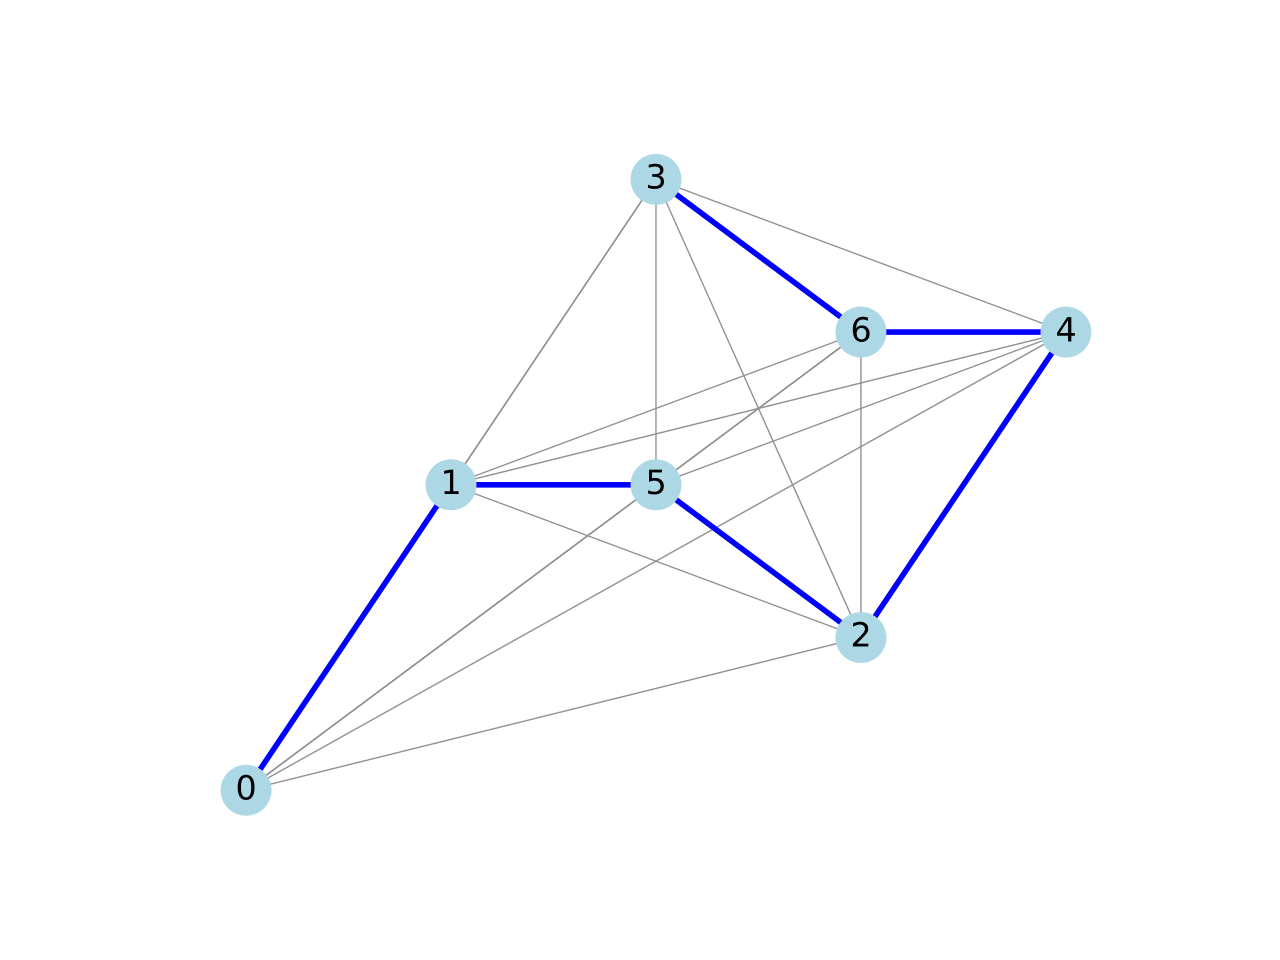
\includegraphics[scale=1]{best_path_arbitrary-1.png}}
    \caption{Exemple de graphe repr\'esentant un monde} 
  \end{figure}
Pour faire la distinction entre les monde avec et sans obstacles, nous collectons d'abord la liste des obstacles dans le monde avce obstacles. Puis pour chaque chemin possible dans le graphe,
on v\'erifie si celui-ci traverse un obstacle.Si c'est le cas, nous augmentons considérablement le poids du chemin.
Afin de r\'pondre au problème posé, nous utiliserons l'algorithme qui permet de résoudre le problème du voyageur de commerce (TSP - travelling salesman problem) par la fuorce brute. L'id\'ee est d'\'enum\'erer toutes 
les permutations possibles des positions des d\'echets et de calculer le co\^ut de chaque permutation pour trouver la permutation avec le co\^ut minimal. Par exemple, si nous avons trois d\'echets 1, 2 et 3, nous pourrions \'enum\'erer toutes les six permutations possibles (123, 132, 213, 231, 312, 321) et calculer le co\^ut de chaque permutation pourt trouver la permutation avec le co\^ut minimum
Cet algorithme garantit le fait de trouver une solution optimale, mais le nombre de permutations cro\^it rapidement avec le nombre de d\'echets \`a ramasser. Par exemple, pour 10 d\'echets, il y a plus de 3,6 millions permutations possibles. Ainsi, l'algorithme force brute reste inefficace pour les instances de grande taille. \\

  \begin{algorithm}[H]
    \SetAlgoLined
    \KwResult{Le meilleur chemin pour rammasser les déchets}
    permutations = allPermutations(n)\;
    bestPath = []\;
    minLength = $\infty$ \;
    \For{i from 0 to longueur(permutations)}
    {
        \If{permLength(permutations[i]) $<$ minLength}
        {
            minLength = permLength(permutations[i])\;
            bestPath = permutations[i]\;
        }
    }
    return bestPath\;
    \caption{bruteForce()}
  \end{algorithm}

  La compl\'exit\'e de cet algorithme est exponentiel de l'ordre $\theta(n!)$



\section{Nos algorithmes solutions}

Afin de résoudre ce problème de manière optimale nous nous sommes posé la question suivante : Comment trouver le chemin de rammassage optimal ?

Une solution évidente est de calculer tous les chemins possibles et de choisir le plus court. Si les $n$ déchets sont représentés par une suite sans répétition de nombre entre 1 et $n - 1$ et la position de départ par le sommet 0, on peut conclure qu'il faut calculer la longueur du chemin parcouru pour toute permutation de l'ensemble $[1 ; n]$.

Ainsi nous définissons les fonctions auxiliaires suivantes : \\

\begin{algorithm}[H]
  \SetAlgoLined
  \KwResult{Un tableau contenant toutes les permutations de [1 ; n]}
  \caption{allPermutations(n)}
\end{algorithm}

\begin{algorithm}[H]
    \SetAlgoLined
    \KwResult{Le temps que le robot prendra pour parcourir la permutation}
    time = 0\;
    currentVector = [0;1]\;
    \For{i from 0 to longueur(permutation) - 1}{
        time = time + poid(i, i+1)\;
        newVector = [pos[i][0] - pos[i+1][0] ; pos[i][1] - pos[i+1][1]]\;
        time = C * angle(currentVector, newVector)\;
        currentVector = newVector\;
    }
    return time\;
    \caption{permLength()}
  \end{algorithm}


  Cependant, on constate rapidement que cette approche a ses limites. En effet, le nombre de permutation pour un ensemble de taille $n$ est $!n$. La complexité en temps et en mémoire de notre alogrithme est donc de $O(n!)$.

  Bien qu'il soit possible de réduire la complexité en espace en fonction de l'implémentation selon un language donné, en utilisant par exemple un itérateur en Python. La complexité en temps, elle, restera inchangée.

  Afin de trouver un autre algorithme, nous nous sommes demandé s'il n'existait pas déjà un problème documenté auquel nous pourrions ramener le nôtre.

  Et, en effet, il est possible de ramener ce problème du rammassage de dechets au problème connu du voyageur de commerce.

  Il existe de nombreux algorithmes permettant de résoudre ce problème, et nous nous sommes interressé à l'algorithme de Christofides.
  
  L'algorithme de Christofides donne une approximation de la solution du marchand de commerce.

  Nous avons donc décidé d'utiliser une variante de celui-ci. En effet, l'algorithme de Christofides consiste à chercher l'arbre couvrant de poid minimum d'un graphe, puis d'effectuer un traitement sur celui-ci.


  Cependant, nous allons simplement effectuer un parcours en profondeur du graphe, et ajouter les sommets dans l'ordre de ce parcours.

%% Donner l'algo. Normalement il n'est pas nécessaire de décrire les algos de calcul de l'arbre couvrant minimal (Prim ou Kruskal) et de parcours en profondeur, car ils sont détaillé dans le cours.

  Cependant, la solution obtenue par cette méthode n'est pas très satisfaisante et il est possible de très simplment améliorer ce résultat. \\ 

  En effet il existe une optimisation possible pour le problème du marchand de commerce, l'algorithme 2-optimisation.

  Cet algorithme consiste à chercher avec une heuristique une solution initiale de chemin le plus court, puis pour tout couple d'arêtes qui se croisent de vérifier le poid du chemin. Si décroiser les arêtes forme un meilleur chemin on continue.

  Cet algorithme se comporte en $\theta (n^2)$ sur la plupart des graphes et donc est plus rapide que l'algorithme "brute force", mais il n'assure absolument pas d'obtenir le chemin optimal, seulement une approximation minimale de ce chemin.\\
  \newline
  \begin{algorithm}[H]
    \SetAlgoLined
    \KwResult{Algo optimisé pour recherche de chemin}
    n = len(solution)\;
    amelioration = True\;
    \While{amelioration == True}{
       meilleur\_gain = 0\;
       amelioration = False\;
       \For{i in range(1,n-2}{
          \For{j in range (i+1,n-1)}{
            gain = G[solution[i-1]][solution[j]]["weight"] + G[solution[i]][solution[j+1]]["weight"] - G[solution[i-1]][solution[i]]["weight"] - G[solution[j]][solution[j+1]]["weight"]\;
            \If{if gain < meilleur\_gain}{       
                  # Inversion des sous-tournées entre i et j
              solution[i:j+1] = reversed(solution[i:j+1])\;
              meilleur\_gain = gain\;
              amelioration = True\;
            }
          }
       }
    }\;
    return solution\;
    \caption{tsp\_2opt(solution,G)}
  \end{algorithm}[H]
%% Basez vous sur le code en python + articles Wikipédia (2-optmisation problème marchand de commerce)

  En effet, dans le parcours obtenue, certaines arrêtes peuvent être croisé, ce qui n'est pas optimal. Ainsi, en décroisant celles-ci, on obtient un bien meilleur résultat.

\end{document}
